%!TeX program = xelatex
%Do not change
\documentclass[12pt, oneside]{article}
\usepackage{amssymb,amsmath}
\usepackage[margin=1in]{geometry}
\usepackage{textpos}
\usepackage{float}
\usepackage{booktabs}
%\usepackage{color}
\usepackage{graphicx}
\usepackage[inter-unit-product =\cdot]{siunitx}
\let\DeclareUSUnit\DeclareSIUnit
\let\US\SI
\DeclareUSUnit\inch{in}
\DeclareUSUnit\foot{ft}
\DeclareUSUnit\mile{mi}
\DeclareUSUnit\foot{ft}
\DeclareUSUnit\slug{slug}
\DeclareUSUnit\pound{lb}
\DeclareUSUnit\psi{psi}
\DeclareUSUnit\Msi{Msi}
\DeclareUSUnit\ksi{ksi}

%\usepackage{tikz}
%\usetikzlibrary{positioning}
%\usepackage{tikz-3dplot}
%\usepackage{pgfopts}
%\usepackage{wasysym}
%\usepackage{stanli}

% You may add the packages you need here
\begin{document}

%TODO change numbers in problems
\begin{textblock*}{4cm}(-1.7cm,-2.3cm)
\noindent {\scriptsize AE333 Fall 2020}
\end{textblock*}

%Do not modify other than putting your name where stated
\begin{textblock*}{8cm}(12.5cm,-1cm)
\noindent {Name: }
\end{textblock*}
%Do not modify other than typing your acknowledgement where stated
\begin{textblock*}{13.5cm}(-1.7cm,-1.8cm)
%\noindent \textit{\footnotesize Acknowledgement: Your acknowledgement for collaboration and other sources goes here. }
\end{textblock*}

\vspace{1cm}

%Do not modify other than typing the homework number after #
\begin{center}
\textbf{\Large Homework 5}

\textbf{Due 29 Sep 2020}
\end{center}

\begin{enumerate}
	\item %P6-1 f
		Draw a free-body diagram of the beam and sketch the general shape of the shear-moment diagram
		\begin{figure}[H]
			\centering
			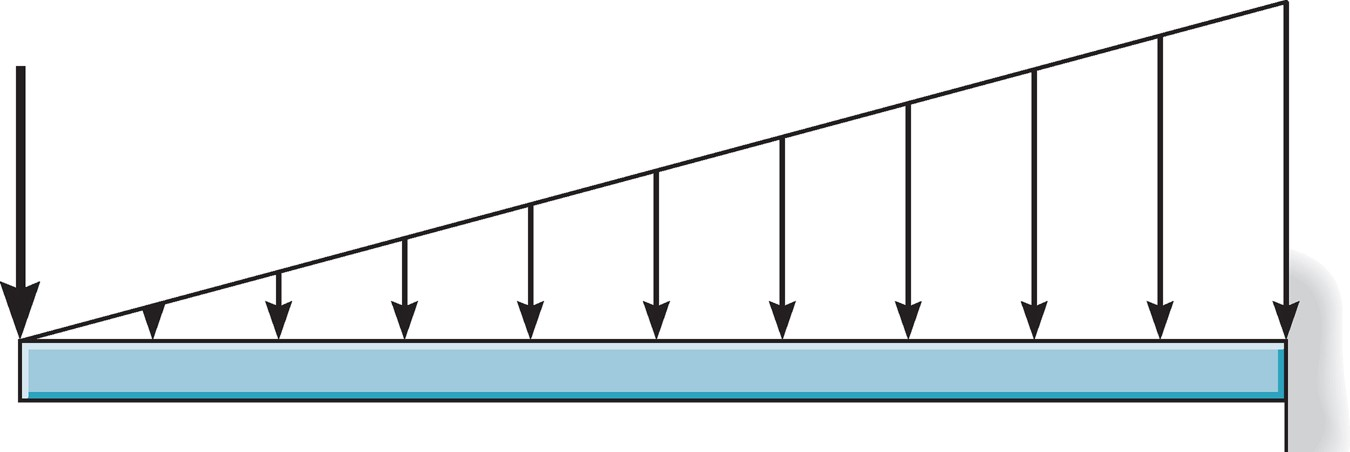
\includegraphics[width=0.6\linewidth]{p6-1f}
		\end{figure}
	\item %6-4
		Draw the shear-moment diagram for the simply supported beam
		\begin{figure}[H]
			\centering
			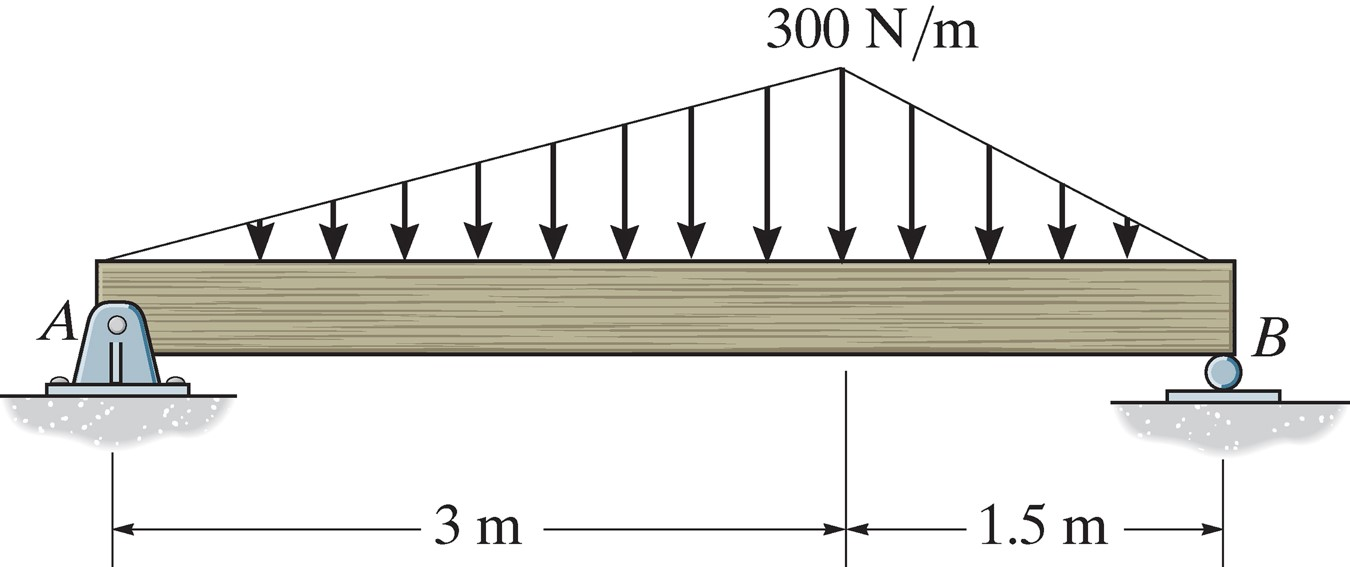
\includegraphics[width=0.6\linewidth]{6-4}
		\end{figure}
	\item %6-15
		Members $ABC$ and $BD$ are rigidly connected at $B$ while the smooth collar at $D$ is allowed to move along the vertical post.
		Draw the shear-moment diagram for $ABC$.
		\begin{figure}[H]
			\centering
			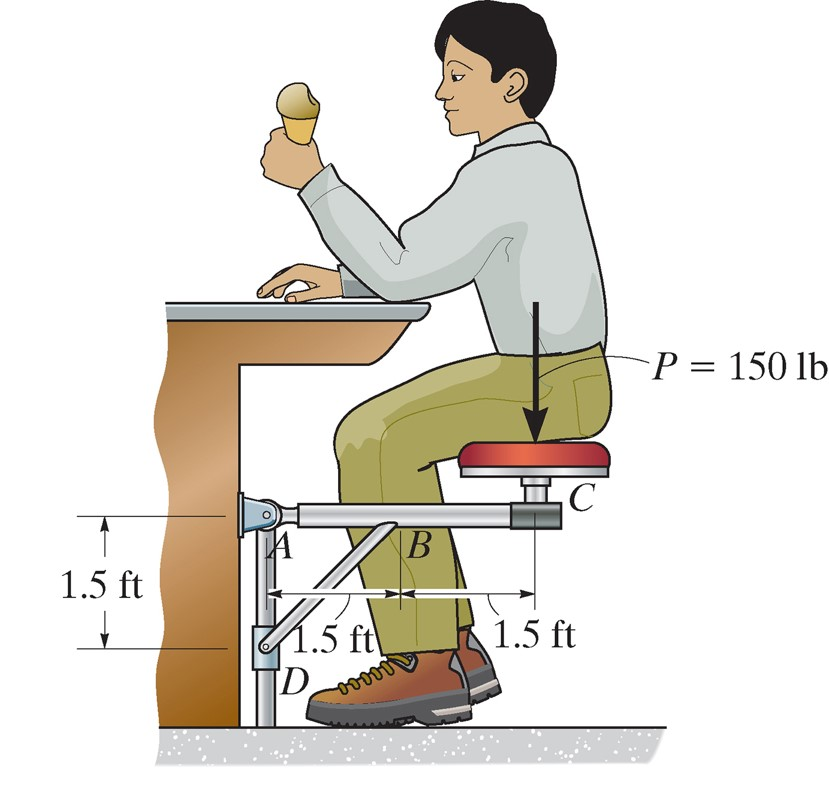
\includegraphics[width=0.3\linewidth]{6-15}
		\end{figure}
		\newpage
	\item %F6-12
		If the beam is subjected to a bending moment of $M=\SI{10}{kN.m}$ find the bending stress in the beam at points $A$ and $B$
		\begin{figure}[H]
			\centering
			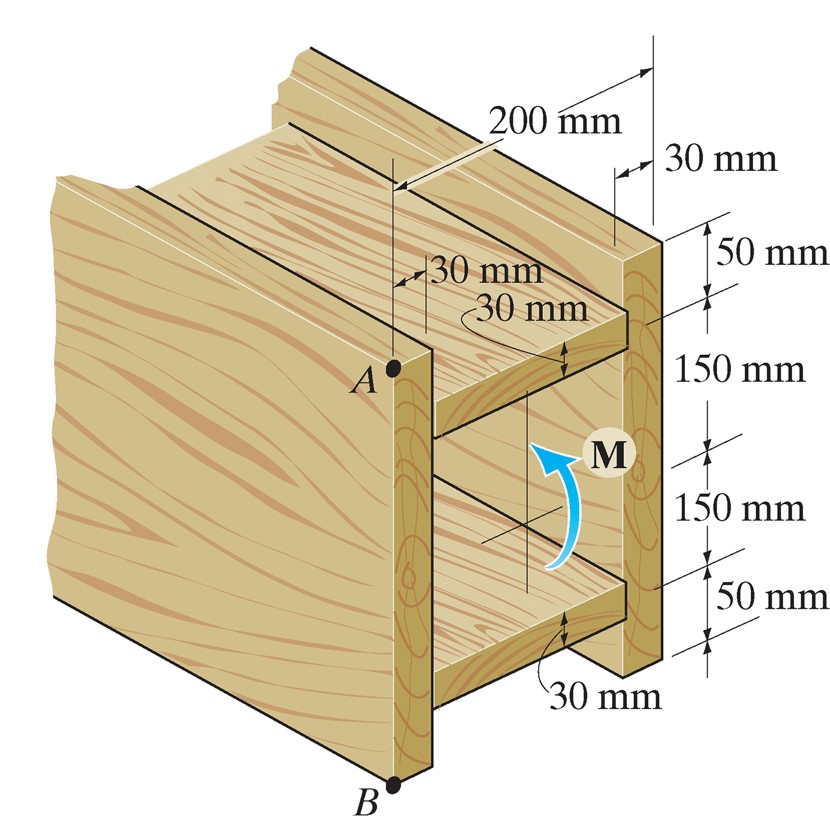
\includegraphics[width=0.5\linewidth]{f6-12}
		\end{figure}
	\item %6-93
		Find the absolute maximum bending stress in the beam assuming that the support at $B$ exerts a uniformly distributed reaction on the beam.
		The cross section is rectangular with a base of $\US{3}{in}$ and a height of $\US{5}{in}$
		\begin{figure}[H]
			\centering
			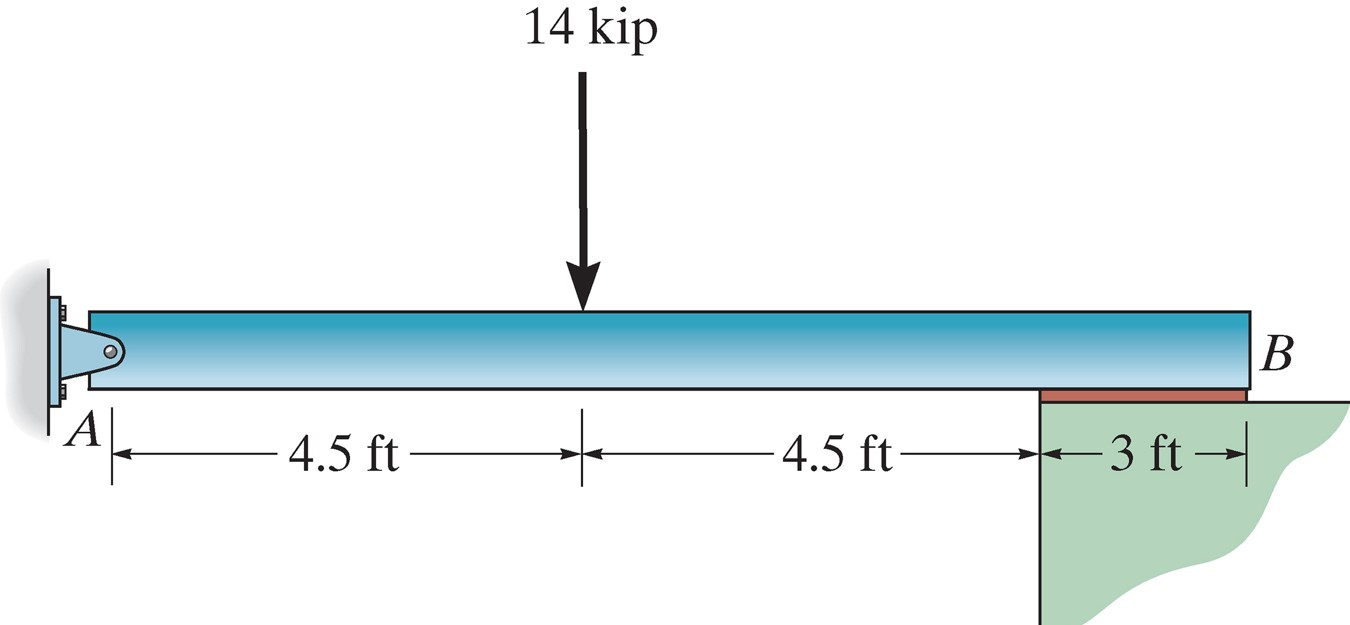
\includegraphics[width=0.6\linewidth]{6-93}
		\end{figure}
		\newpage
	\item %6-101
		If the allowable bending stress is $\sigma_{allow} = \SI{6}{MPa}$, find the maximum dimension, $d$ of the beams cross sectional area.
		\begin{figure}[H]
			\centering
			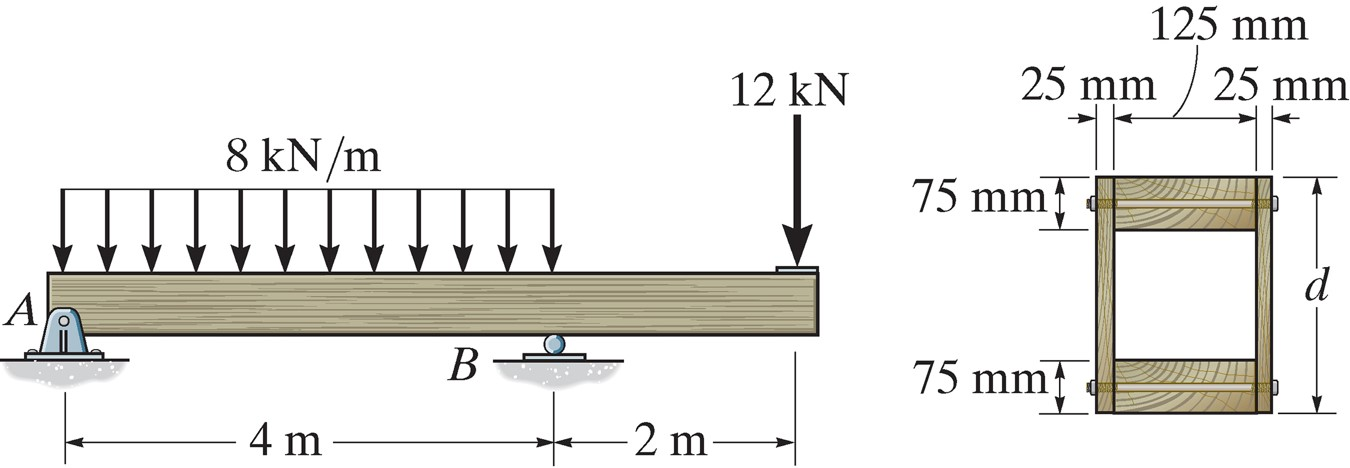
\includegraphics[width=0.8\linewidth]{6-101}
		\end{figure}
	\item %C6-4
		These garden shears were manufactured using an inferior material.
		Using a load of $\US{50}{lb}$ and appropriate dimensions find the maximum bending stress and show why failure occurred at this location
		\begin{figure}[H]
			\centering
			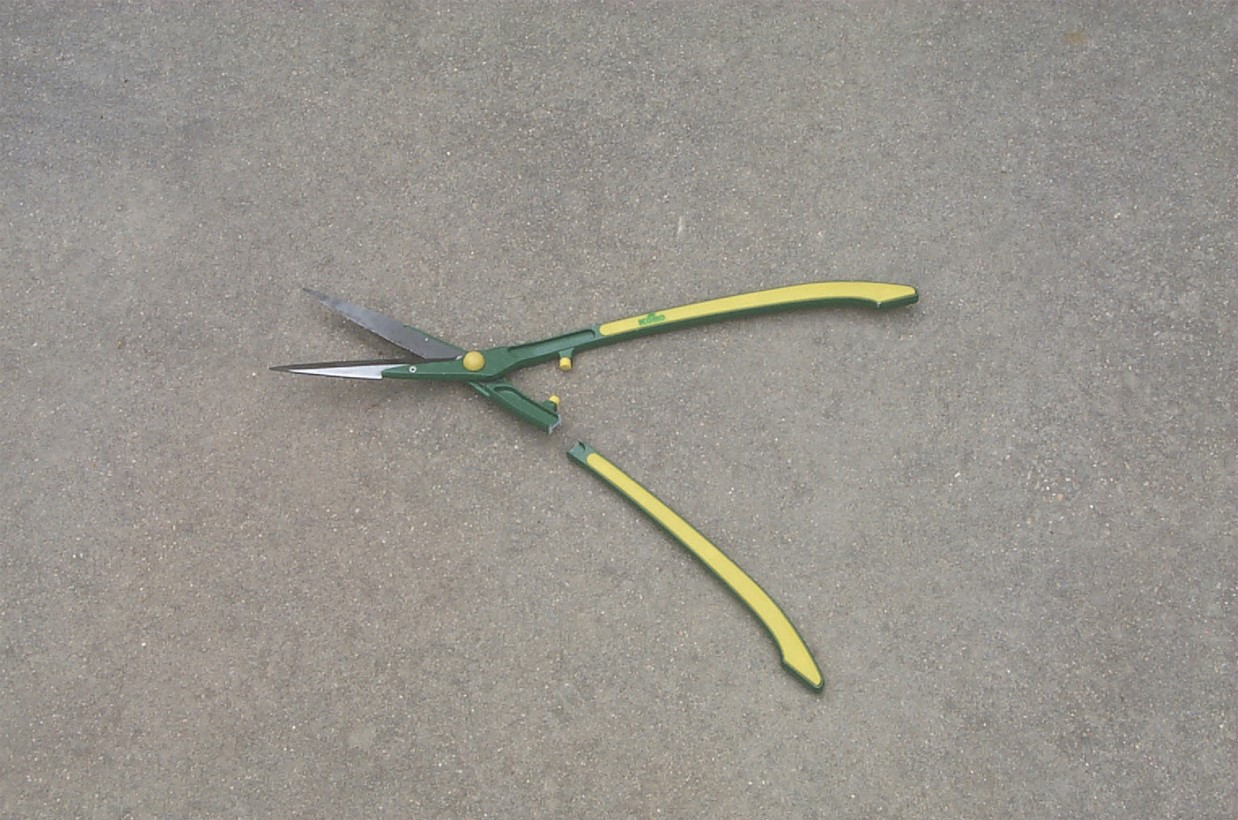
\includegraphics[width=0.7\linewidth]{c6-4a}
		\end{figure}
		\begin{figure}[H]
			\centering
			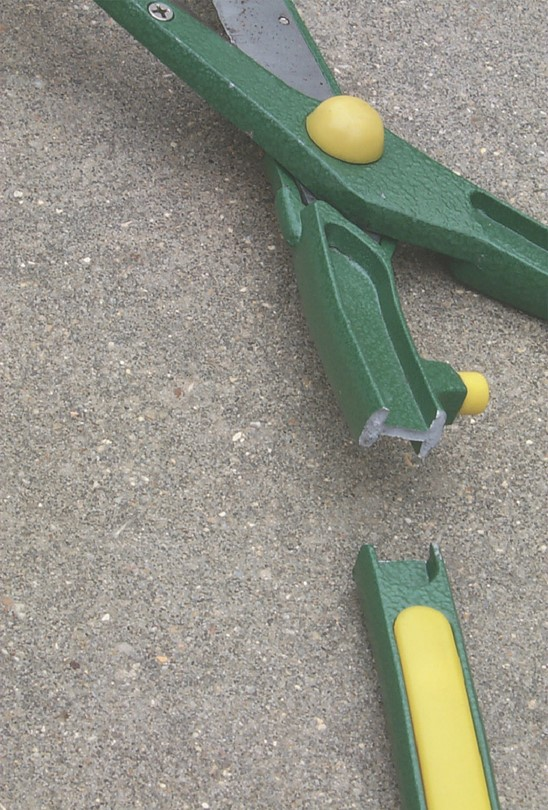
\includegraphics[width=0.4\linewidth]{c6-4b}
		\end{figure}
\end{enumerate}
\end{document}
